\documentclass[aps,prl,preprint,groupedaddress]{revtex4-2}
\usepackage{mhchem, siunitx}

\begin{document}
\title{Measuring the Planck Constant from the Minimum Wavelength of X-rays in the Bremsstrahlung Continuum}
\author{Tom Falcone}
\affiliation{Department of Physics, Temple University}
\date{\today}
\begin{abstract}
    The aim of the experiment was to verify the Duane-Hunt relation by measuring the minimum wavelengths of the bremsstrahlung continuum associated with a several different voltages. With that, we could calculate the Planck constant by determining a general formula for minimum wavelength as a function of voltage. Our results support the Duane-Hunt relation, and we measured $h = 6.52(5) \times 10^{-34} ~\si{J.s}$.
\end{abstract}
\maketitle
\section{Introduction}
    In 1915, William Duane and Franklin Hunt measured the minimum wavelength of x-rays in the bremsstrahlung continuum associated with a constant voltage $U$.~\cite{duane} This meant that the energy of any emitted x-ray was bounded above by the energy of a single colliding electron, which served to corroborate early quantum theory. By measuring this limit wavelength for several different $U$, they established that $\lambda_{min} \propto \frac{1}{U}$ with constant of proportionality $A = \frac{h c}{e}$. In turn, they measured the Planck constant to be $6.39 \times 10^{-34}~\si{J.s}$, an accurate measurement for the time that we aimed to improve upon.
\section{Experimental Method}
    In an x-ray tube, electrons are produced by a hot tungsten filament and accelerated through a potential difference $U$ en route to a molybdenum (\ce{Mo}) target. A continuous distribution of x-rays with frequencies ranging from $0$ to $\nu_{max}$
    are produced via bremsstrahlung. Then, the x-rays pass through a collimator that directs them onto a monocrystal of \ce{NaCl}, which, together with a counter tube, is attached to a goniometer. Only x-rays of a particular wavelength scatter off of the \ce{NaCl} lattice planes in such a way that they are "reflected" toward the counter tube. Once in the G-M-tube, the radiation of the x-rays is calculated and sent to the computer. In evenly parsed intervals, the \ce{NaCl} and the counter tube are rotated with respect to the incoming x-ray beam in $2\theta$ coupling, allowing x-rays with wavelengths over a representative portion of the bremsstrahlung continuum to be collected. The software on the computer plots radiation, $R$, in $\si{s^{-1}}$, against wavelength,  $\lambda$, in $\si{pm}$. We completed this process $8$ times for $U = 22, 24, \ldots, 34$ and $U = 35$, where $U$ is in $\si{kV}$, each time producing a curve in the software. For each curve, we constructed the line of best fit and recorded the wavelength of this line corresponding to $0$ radiation, i.e. the minimum wavelength.
\section{Theoretical Background}
    The electrons have energy $E_e = eU$ on impact. When the electrons collide (i.e. enter the \ce{Mo} target) they are rapidly decelerated by the positively charged \ce{Mo} atoms. This deflection results in the production of a photon. Both the EM radiation resulting from the creation of photons (x-rays in this case) and the process itself are known as bremsstrahlung. Since a deflected electron can give up at most all of its energy to a photon, and the energy of any x-ray is given by $E = h\nu$, the frequency of the x-rays has an upper bound ($\nu_{max}$), and the wavelength a lower bound ($\lambda_{min}$):
    \begin{align}
        \nu_{max} &= \frac{e}{h}U\\
        \lambda_{min} &= \frac{hc}{e}\frac{1}{U}
    \end{align}
    Thus, the bremsstrahlung continuum for a particular voltage $U$ consists of x-rays with wavelength in the interval $(\frac{hc}{e}\frac{1}{U}, \infty)$. When the x-rays collide with the \ce{NaCl} monocrystal, they scatter in all directions, so only those x-rays that constructively interfere in the direction of the counter tube are measured. According to the Bragg condition of first order, these measured x-rays must satisfy
    \begin{align}
        \lambda = 2 d sin(\theta),
    \end{align}
    where $d = 282.01~\si{pm}$ is the lattice plane spacing of NaCl. So, wavelength is determined by the angle $\theta$ of the monocrystal with respect to the beam of x-rays. After the software plots the radiation vs. wavelength curves and calculates $\lambda_{min}$ for each $U$ value, we can use the voltage and minimum wavelength data to calculate the least squares regression line
    \begin{align}
        \lambda_{min} = A \frac{1}{U}~.
    \end{align}
    Finally, equations (2) and (4) can be used to calculate 
    \begin{align}
        h = \frac{e}{c} A~.
    \end{align}
    
	\begin{figure}
		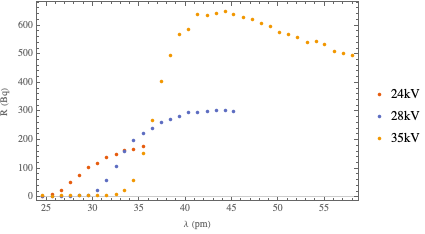
\includegraphics{rad_data.png}
		\caption{Each set of points represents the
		                beginning of the bremsstrahlung continuum for a particular voltage,
		                given by the legend.}
	\end{figure}
	\begin{figure}
		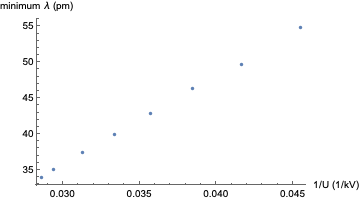
\includegraphics{min_wavelength.png}
		\caption{Here, we have the minimum wavelength 
		        corresponding with each voltage.}
	\end{figure}
\section{Results}
A sample of the data collected is given in FIG 1. We can see that the data is qualitatively consistent with the smooth curve of the bremsstrahlung continuum. The minimum wavelength data for each $U$ value is shown in FIG 2. By performing the method of least squares on the data in FIG 2., we calculated $A = 1.22(1) \times 10^{-6}~\si{J.m}$. By using the accepted values~\cite{mohr} of $c = 299~792~458~\si{m.s^{-1}}$ and $e = 1.602~176~6208(98) \times 10^{-19}~\si{C}$ (and also noting that the error in $e$ is negligible for our purposes), we use equation (5) and propagate the error in $A$ to compute $h = 6.52(5) \times 10^{-34}~\si{J.s}$. The currently accepted value of the Planck constant is $h = 6.626~070~040(81) \times 10^{-34}~\si{J.s}$ While not without fault, our calculation is indeed more accurate than the value calculated in the Duane-Hunt experiment.
\section{Discussion}
The results from our experiment are consistent with the Duane-Hunt relation, and, from these data, we were able to calculate the Planck constant with reasonable accuracy. Some aspects of the experiment could be improved. An increase in the range of rotation of the goniometer may improve in detecting small wavelengths, especially considering that trials 6, 7, and 8 all had readings for wavelengths at $24.6~\si{pm}$ the shortest wavelength our apparatus can detect, and, therefore, the smallest angle between the monocrystal and the x-ray beam. By placing the counter tube slightly closer to the monocrystal we may also be able to detect more radiation. Another improvement could be made by measuring the actual lattice plane spacing of the \ce{NaCl} beforehand, thereby adding a layer of quality control. Beyond natural impurities, the \ce{NaCl} is very delicate, and any faults in the material, or possible absorption of water vapor, would result in incorrect measurements of any $\lambda$, and also $\lambda_{min}$, which accounts for some of the discrepancy between the calculated h and the accepted value.
\bibliography{resources.bib}
\end{document}
